\chapter{Introduction}\label{Chap1}
\echapter{Introduction}
In the microelectronics industry, the chip technology is rapidly evolving towards miniaturization in accordance to the Moore's law. Owing to this miniaturization trend in the chip technology, the reliability of solder joints used in the electronic packaging has been considered as a significant topic.  Among the several aspects of reliability, the microbubbles and intermetallic compounds(IMCs), which get formed and grow considerably during the reflow soldering need special attention. With the dimensions of these bubbles being several values lower than millimeters length scale, the experimental study need to assisted by computational methods for a better understanding of the physical properties and phenomena.

\section{Background}\label{Chap1_01}
\esection{Background}

\subsection{Planar Microbubbles} \label{Chap1_01_01}
\esubsection{Planar Microbubbles}
Solder voiding has been a common phenomenon in mass reflow soldering processes used in the electronic packaging technologies, being variously characterized as process anomalies, process indicators and/or solder defects. A solder void can be defined as a hole or enclosed volume of space within the solder joint that lacks solder material ~\cite{TLLewis:2012}. The planar microbubbles or microvoids, having size smaller than 1-2 millimeters in diameter and being located in one plane at the substrate-to-solder interface above the intermetallic compound, are considered to be the risk for reliability failures of BGA and other solder joints ~\cite{RAspandiar:2006}. Most of the cases of planar microbubbles are associated with the gaseous materials resulting from the flux during reflow soldering.

\subsection{Intermetallic Compounds} \label{Chap1_01_02}
\esubsection{Intermetallic Compounds}
The compounds that are formed at the interface of the Sn rich solder and Cu substrate  are called the intermetallic compounds (IMCs). Cu$_6$Sn$_5$ and Cu$_3$Sn are the commonly known IMCs in the Sn and Sn-0.7Cu solder system.  Owing to the brittle nature of these compounds,the thickness of the IMC is considered an important reliability parameter ~\cite{MLHuang2015}. For most of the design purpose, solder systems are supposed to have a relatively thinner IMC.



\section{Motivation}\label{Chap1_01}
\esection{Motivation}
As most of the electronic devices are undergoing the trend of miniaturization, study of the reliability issues in electronic packaging assemblies and solder joints has acquired a notable significance among the researchers.As the solder microvoids, decrease the contact area of the solder interface and weaken the solder joints, they are the one of the key issues regarding the reliability of solder joints. The simulation of the growth behavior of solder bubbles and voids through computational methods can be a good approach when the experimental study about the solder voiding is at the crossroads. In relation to the IMCs of solder joints in real practice, the phenomena of thermomigration and electromigration interfere the growth pattern of the compounds. Thus, the assessment of the dimensional changes of the IMCs under the externally applied temperature  and electric field  gradients can contribute to the knowledge of design parameters in soldering procedures. In this connection, the implementation of numerical models can assist in better  as well as meticulous understanding of the physical phenomena and material properties.

\section{Problem Statement}\label{Chap1_01}
\esection{Problem Statement}
With respect to the study of the solder microvoids and intermetallic compounds in microelectronic packaging, the following statements can be written in order to outline as the major research objectives:
\begin{enumerate}
\item To model the diffusion driven growth of single and multiple bubbles in liquid Sn based solders. 
\item To measure and numerically calculate the thickness of Cu$_6$Sn$_5$ at the anode of Cu/liquid Sn/Cu solders undergoing electromigration.
\item To measure and numerically calculate the thickness of Cu$_6$Sn$_5$ at the cold side of Cu/liquid Sn/Cu solders undergoing thermomigration. In addition, the experimental evaluation of the IMC thickness is done for liquid Sn-3.5Ag solders
\end{enumerate}

It is to be noted that the present work is done for the analysis of thickness of Cu$_6$Sn$_5$ IMC owing to the limitation imposed in the experimental measurements of the very thin Cu$_3$Sn compound. For further reference, the abbreviation IMCs refers to Cu$_6$Sn$_5$ compound unless otherwise stated. 

\section{Summary of Research Contributions}\label{Chap1_02}
\esection{Summary of Research Contributions}

The innovative contributions of this dissertation, which are elaborated throughout this dissertation, are listed as follows:
\begin{enumerate}
    \item \textbf{Modeling of Microbubbles in Liquid Sn Solders}
    \\
   Finite element method is utilized to solve the diffusion equation and model the diffusion driven growth of a pre-existing spherical gas bubble in molten tin at the solder/substrate interface for reflow time of 120 s and temperature of 250 °C. The gibbs free energy change required for determining the equilibrium concentration at liquid solder/gas bubble boundary was calculated using the thermodynamic polynomial coefficients. The rate of change of radius, as function of concentration flux, is calculated using the lagrangian mesh update methodology. With an initial diameter of 20 μm, the bubble growth is calculated as a function of contact angle. When the wetting angle is varied from a value of 30° to 135°, the numerical calculation has yielded the final sizes for the bubble to change from 62.87 μm to 82.8 μm respectively. The effect of wetting transition in the growth of bubble was studied by the in-situ observation of bubble dynamics through synchrotron radiation imaging technique. The scanning electron microscopy images of the morphologies of intermetallic compounds influenced by growing bubble in Sn/Cu solder joint and bubble pictures obtained through synchrotron radiation are utilized to get the experimental size of the bubble. The mean experimental bubble diameter has been obtained as 76.39 μm. The growing bubble inhibits the growth of intermetallic compound at its vicinity and thereby reduces the strength of solder joints.
    \item \textbf{Observation of the thickness increase of IMC at the anode of Cu/liquid Sn/Cu under electric field gradient}
    \\
    Synchrotron radiation imaging technology was applied for in situ observation of the growth of Cu6Sn5 intermetallic compounds at the anode in Cu/molten Sn/Cu joint undergoing electromigration. For current density of 0.6 × 103 A/cm2, temperature of 250 °C and reflow heating time of 1 h, thickness of the compound was obtained as 110 μm. The thickness growth was observed to have linear dependence with time. The numerical model for diffusion and electromigration of the copper species was implemented using the finite volume method.
    
    \item \textbf{Study of the thickness increase of IMC at the cold end of Cu/liquid Sn/Cu and Cu/liquid SnAg/Cu under thermal gradient}
    The thermal gradient induced intermetallic compound growth at the cold side of the Cu/Sn/Cu and Cu/Sn-3.5Ag/Cu solders heated at 350° has been in-situ studied using synchrotron radiation imaging technique. Finite element model for thermotransport of Cu from hot end to cold end in Cu/Sn/Cu solder is implemented for the description of the associated growth of the compound. Higher temperature and bigger solder volume are observed as favorable parameters for the rate of thickness increase in both Sn and SnAg solders. In case of SnAg system, the formation of Ag3Sn particle, causing retardation effects in the growth of Cu6Sn5 compound, subsequently induces a lowered resulting thickness.
\end{enumerate}

\section{Organization of the Dissertation}\label{Chap1_03}
\esection{Organization of the Dissertation}
\begin{figure}[h]
\begin{center}
  \begin{tabular}{c}
  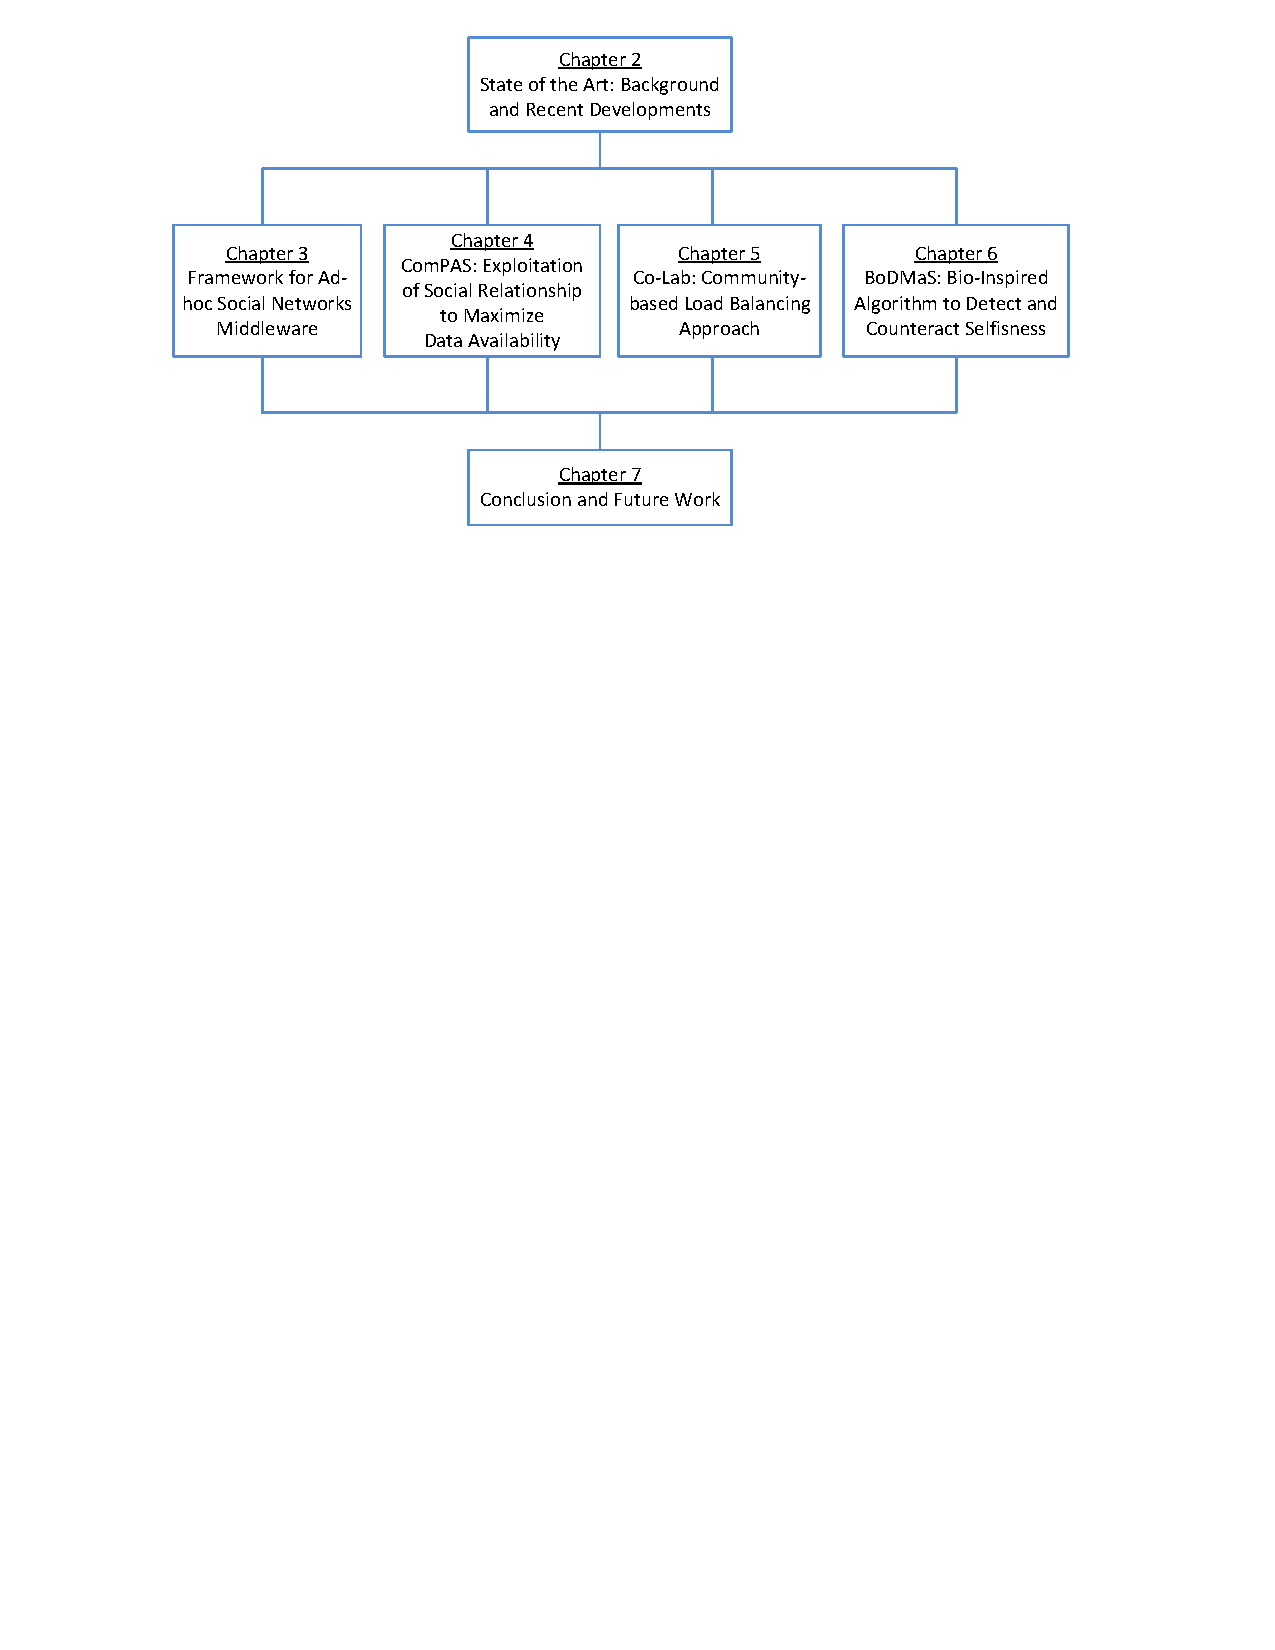
\includegraphics[width=0.856\textwidth]{Chap1-Fig2.pdf}
  \end{tabular}
  \caption{The organization of the remainder of the dissertation.}
\end{center}
\end{figure}
The remainder of the dissertation is organized as shown in Fig. 1.2: Chapter 2 lays a theoretical state of the art background for the following work, including introductions to user social behaviors, user mobility, middleware solutions for ad-hoc social networks, data replication, load balancing and user selfishness. Chapter 3 provides an ASNET middleware framework and overview of the relation of the layers as well as the protocols. Chapter 4 presents a social community partition aware replica allocation scheme that exploits users' relationship. In Chapter 5, we propose an optimal community-based load-balancing method. Chapter 6 provides bio-inspired algorithm to detect and counteract selfishness in ASNETs. Chapter 8 concludes the dissertation and discusses future research directions.

To provide an overall picture of the dissertation content, we created a dependency graph among chapters (Fig. 1.3) in which arrows suggest dependencies between chapters. Based on the dependency graph, therefore, a reader can start with Chapter 2 (state of the art: background and recent developments), and it is recommended that he or she read Chapters 3 (framework for ad-hoc social networks middleware) and 4 (ComPAS) before Chapter 5 (Co-Lab) and Chapter 6 (BoDMaS). We have also color-coded chapter boxes that are of the same level of importance and abstraction. The darkest chapters are the essentials of this dissertation, and the lightest boxes are those chapters that are more applied and have materials that are built on the foundation of other chapters.

\begin{figure}[h]
\begin{center}
  \begin{tabular}{c}
  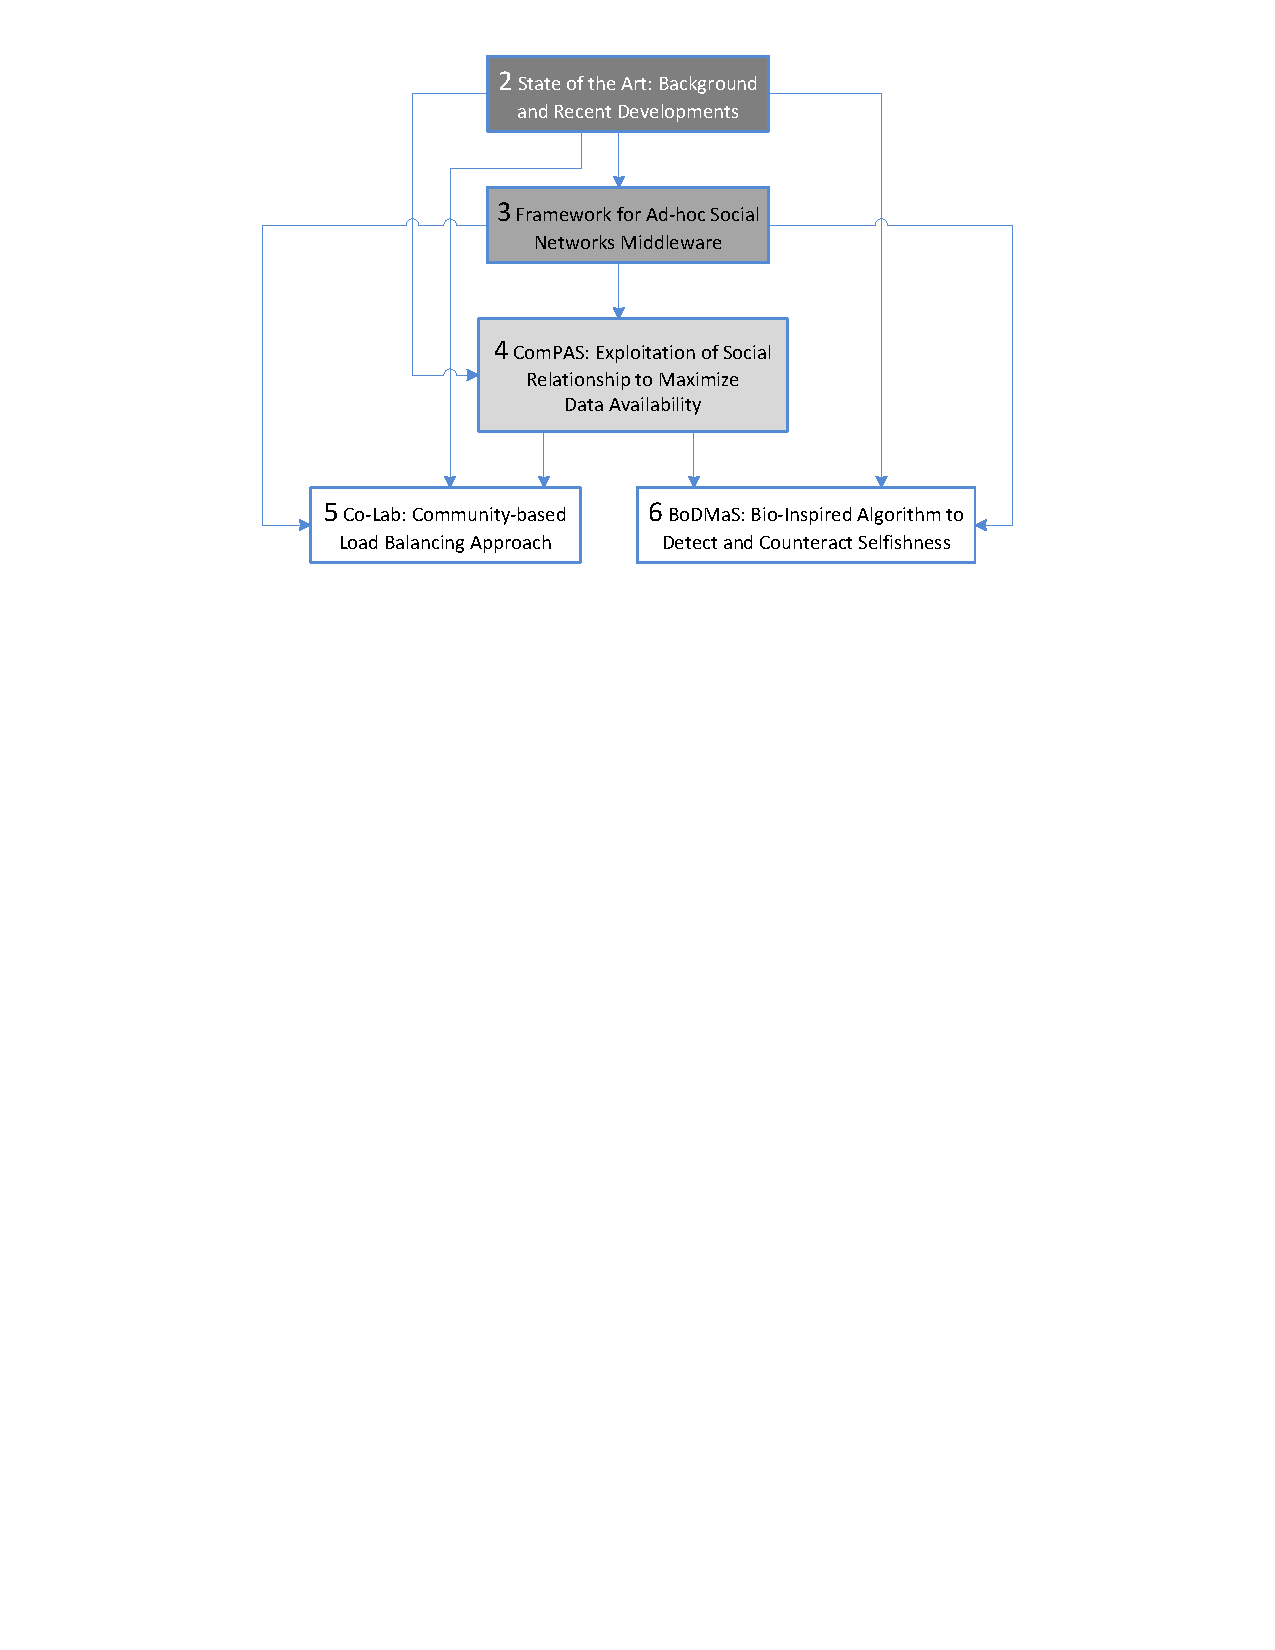
\includegraphics[width=0.75\textwidth]{Chap1-Fig3.pdf}
  \end{tabular}
  \caption{Dependency between dissertation Chapters. Arrows show dependencies and colors represent chapter levels.}
\end{center}
\end{figure}
